\documentclass[screen, aspectratio=169]{beamer}
\usepackage[T1]{fontenc}
\usepackage[utf8]{inputenc}

% Use the NTNU-temaet for beamer 
% \usetheme[style=ntnu|simple|vertical|horizontal, 
%     language=bm|nn|en, 
%     smalltitle, 
%     city=all|trondheim|alesund|gjovik]{ntnu2017}
\usetheme[style=ntnu, language=en, smalltitle]{ntnu2017}

\usepackage[english]{babel}
\usepackage[style=numeric,backend=biber,natbib=false,sorting=none]{biblatex}
\usepackage{hyperref}

\title[PCW-d1]{Physical Computing Workshop: Day 1}
\subtitle{Intuitive Handmade Electronic Music}
\author[A. Xamb{\'o}]{Anna Xamb{\'o}}
\institute[NTNU]{Department of Music, NTNU}
\date{15 October 2019}
%\date{} % To have an empty date

\addbibresource{../pcw.bib} % Add bibliography database

% Set the reference style to numeric.
% See here: http://tex.stackexchange.com/questions/68080/beamer-bibliography-icon
\setbeamertemplate{bibliography item}[text] 

% Set bibliography fonts to a small size.
\renewcommand*{\bibfont}{\footnotesize}

\begin{document}

\begin{frame}
  \titlepage
\end{frame}
%
\begin{frame}
\frametitle{Setting up}
\begin{itemize}
\item Fill in the pre-questionnaire (Canvas)
\item Download material from day 1 (Github)
\item Download and install Puredata Vanilla: \url{https://puredata.info/downloads/vanilla}
\item Create a user account at Freesound.org
\end{itemize}
\end{frame}
%
%
%\begin{frame}
%\frametitle{Schedule}
%\begin{itemize}
%\item 9.15-9.45: BELA kits, forms and visit to the electronic lab
%\item Download material from day 1
%\item Download and install Puredata Vanilla
%\item Create a user account at Freesound.org
%\end{itemize}
%\end{frame}
%

\begin{frame}
\frametitle{Learning Outcomes}
By the end of the session,  you will be able to...
\begin{itemize}
\item Create basic sonic handmade circuits with everyday objects.
\item Explore the practice of circuit sniffing using radios, microphones and speakers.
\item Reflect on this type of recordings by describing their sound properties.
\item Discern the fundamental properties of an interactive musical system.
\item Demonstrate a custom-made sampler instrument in a performance setting.
\item Reflect on the custom-made sampler instrument and performance using a blogging style.
\end{itemize}
\end{frame}
%
\begin{frame}
  \frametitle{Preparation: What to Bring to Class?}
  For the first day, you are welcome to bring (it is likely you can find some of the items in your respective \emph{electronikklabs}, and you can work in teams to complement each other's collections of items):
        \begin{itemize}
	{\tiny 	
	\item a raw loudspeaker of any size (if you have it) -- see photo above
	\item a 9-volt battery
	\item jumper leads with alligator clips (only two will be provided, you will need at least one more)
	\item any type of contact mic, pickup or piezo (if you have it, we will work with them in groups)
	\item a medium size nail
	\item pop-tabs from soda cans, paper clips, nuts and bolts
	\item a can with a smaller diameter than your speaker (if you have it)
	\item some lentils, beans, or gravel (if you have it)
	\item a small piece of aluminium foil (if you have it)
	\item plastic or metal bowls, larger than your speaker, or a toilet plunger (if you have it)
	\item cheap headphones / earplugs
	\item a mobile phone with a radio program or a battery-powered AM radio
	\item a battery-powered amplifier (optional, you will have 1 per group)
	\item a minijack to jack adapter (if you have it, for the battery-powered amplifier)
	\item an audio recording device per group (a mobile phone is accepted)
	}
         \end{itemize}
\end{frame}
%

\usebackgroundtemplate{}
\begin{frame}
%\transcover
\frametitle{}
{\huge Block I\\ The Victorian Synthesizer\\ Circuit Sniffing\\ Soundwalking Activities}
\end{frame}

\begin{frame}
  \frametitle{The seven basic rules of hacking (Collins 2006)}
        \begin{itemize}
	\item Rule \#1: Fear not!
	\item Rule \#2: Don't take apart anything that plugs directly into the wall.
	\item Rule \#3: It is easier to take something apart than put it back together.
	\item Rule \#4: Make notes of what you are doing as you go along, not after.
	\item Rule \#5: Avoid connecting the battery backwards.
	\item Rule \#6: Many hacks are like butterfies: beautiful but short-lived.
	\item Rule \#7: In general, try to avoid short circuits.
    \end{itemize} 
\end{frame}
%
\begin{frame}
  \frametitle{Exercise 1: Loudspeakers with batteries}
   \begin{figure}
	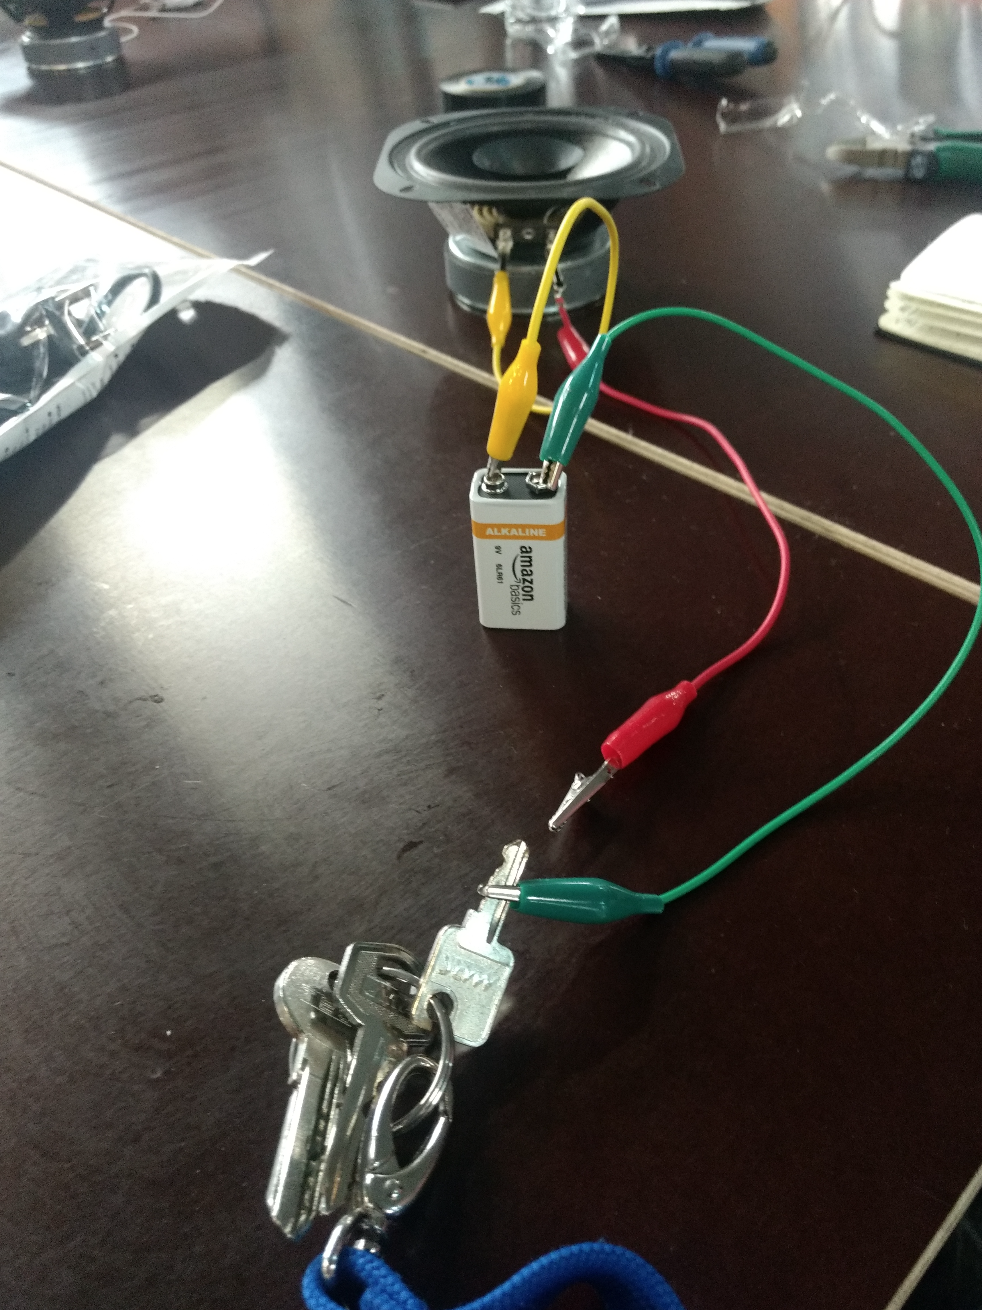
\includegraphics[scale=0.2]{img/loudspeakers-batteries.png}
\end{figure}
{\scriptsize 
Passing the battery current through the speaker coil creates an electromagnet that interacts with the speaker's fixed magnet and moves the cone in or out.\\
}    
{\tiny
Exercise based on ``Chapter 5. The celebrated jumping speaker of Bowers county: Twitching loudspeakers with batteries'' (Collins 2006).
%Video: https://www.youtube.com/watch?v=6ZxxuDNQuMQ&list=PLyFW-rnLqSeGxwsL0FL160g8y6XmdHZcQ&index=3
}
\end{frame}
%
\begin{frame}
  \frametitle{Exercise 1: Loudspeakers with batteries}
 {\scriptsize 
 Passing the battery current through the speaker coil creates an electromagnet that interacts with the speaker's fixed magnet and moves the cone in or out.
   \begin{itemize}
	\item Step 1: Clip 1 from battery terminal (``+'' or ``-'') to loudspeaker terminal. Clip 2 from speaker terminal to battery terminal intermittently.
	\item Step 2: Clip 1 from battery terminal (``+'' or ``-'') to loudspeaker terminal. Clip 2 from speaker terminal to conductive metal. Clip 3 from battery terminal to nail / pointed conductive metal. Touch nail to metal. Send short pulses to keep the battery alive.
	\item Replace the two metal pieces with coins, paperclips, aluminum pop-tabs. Place it inside the speaker cone. Try to change the pitch and rhythm of the buzzing sounds.
	\item Try to connect them in series and in parallel.
	\item Try to use your hands, bowls, and so on, to mute and resonate the sound further. 
	\item Put gravel, coins, or dried lentils inside the cone for additional rhythmic accents. 
	\item Check the Victorian Synthesizer by John Bowels: \url{http://www.jmbowers.net/works/victorian.html}
    \end{itemize}   
}    
{\tiny
Exercise based on ``Chapter 5. The celebrated jumping speaker of Bowers county: Twitching loudspeakers with batteries'' (Collins 2006).
}
\end{frame}
%
\begin{frame}
  \frametitle{Exercise 2: Circuit sniffing}
   \begin{figure}
	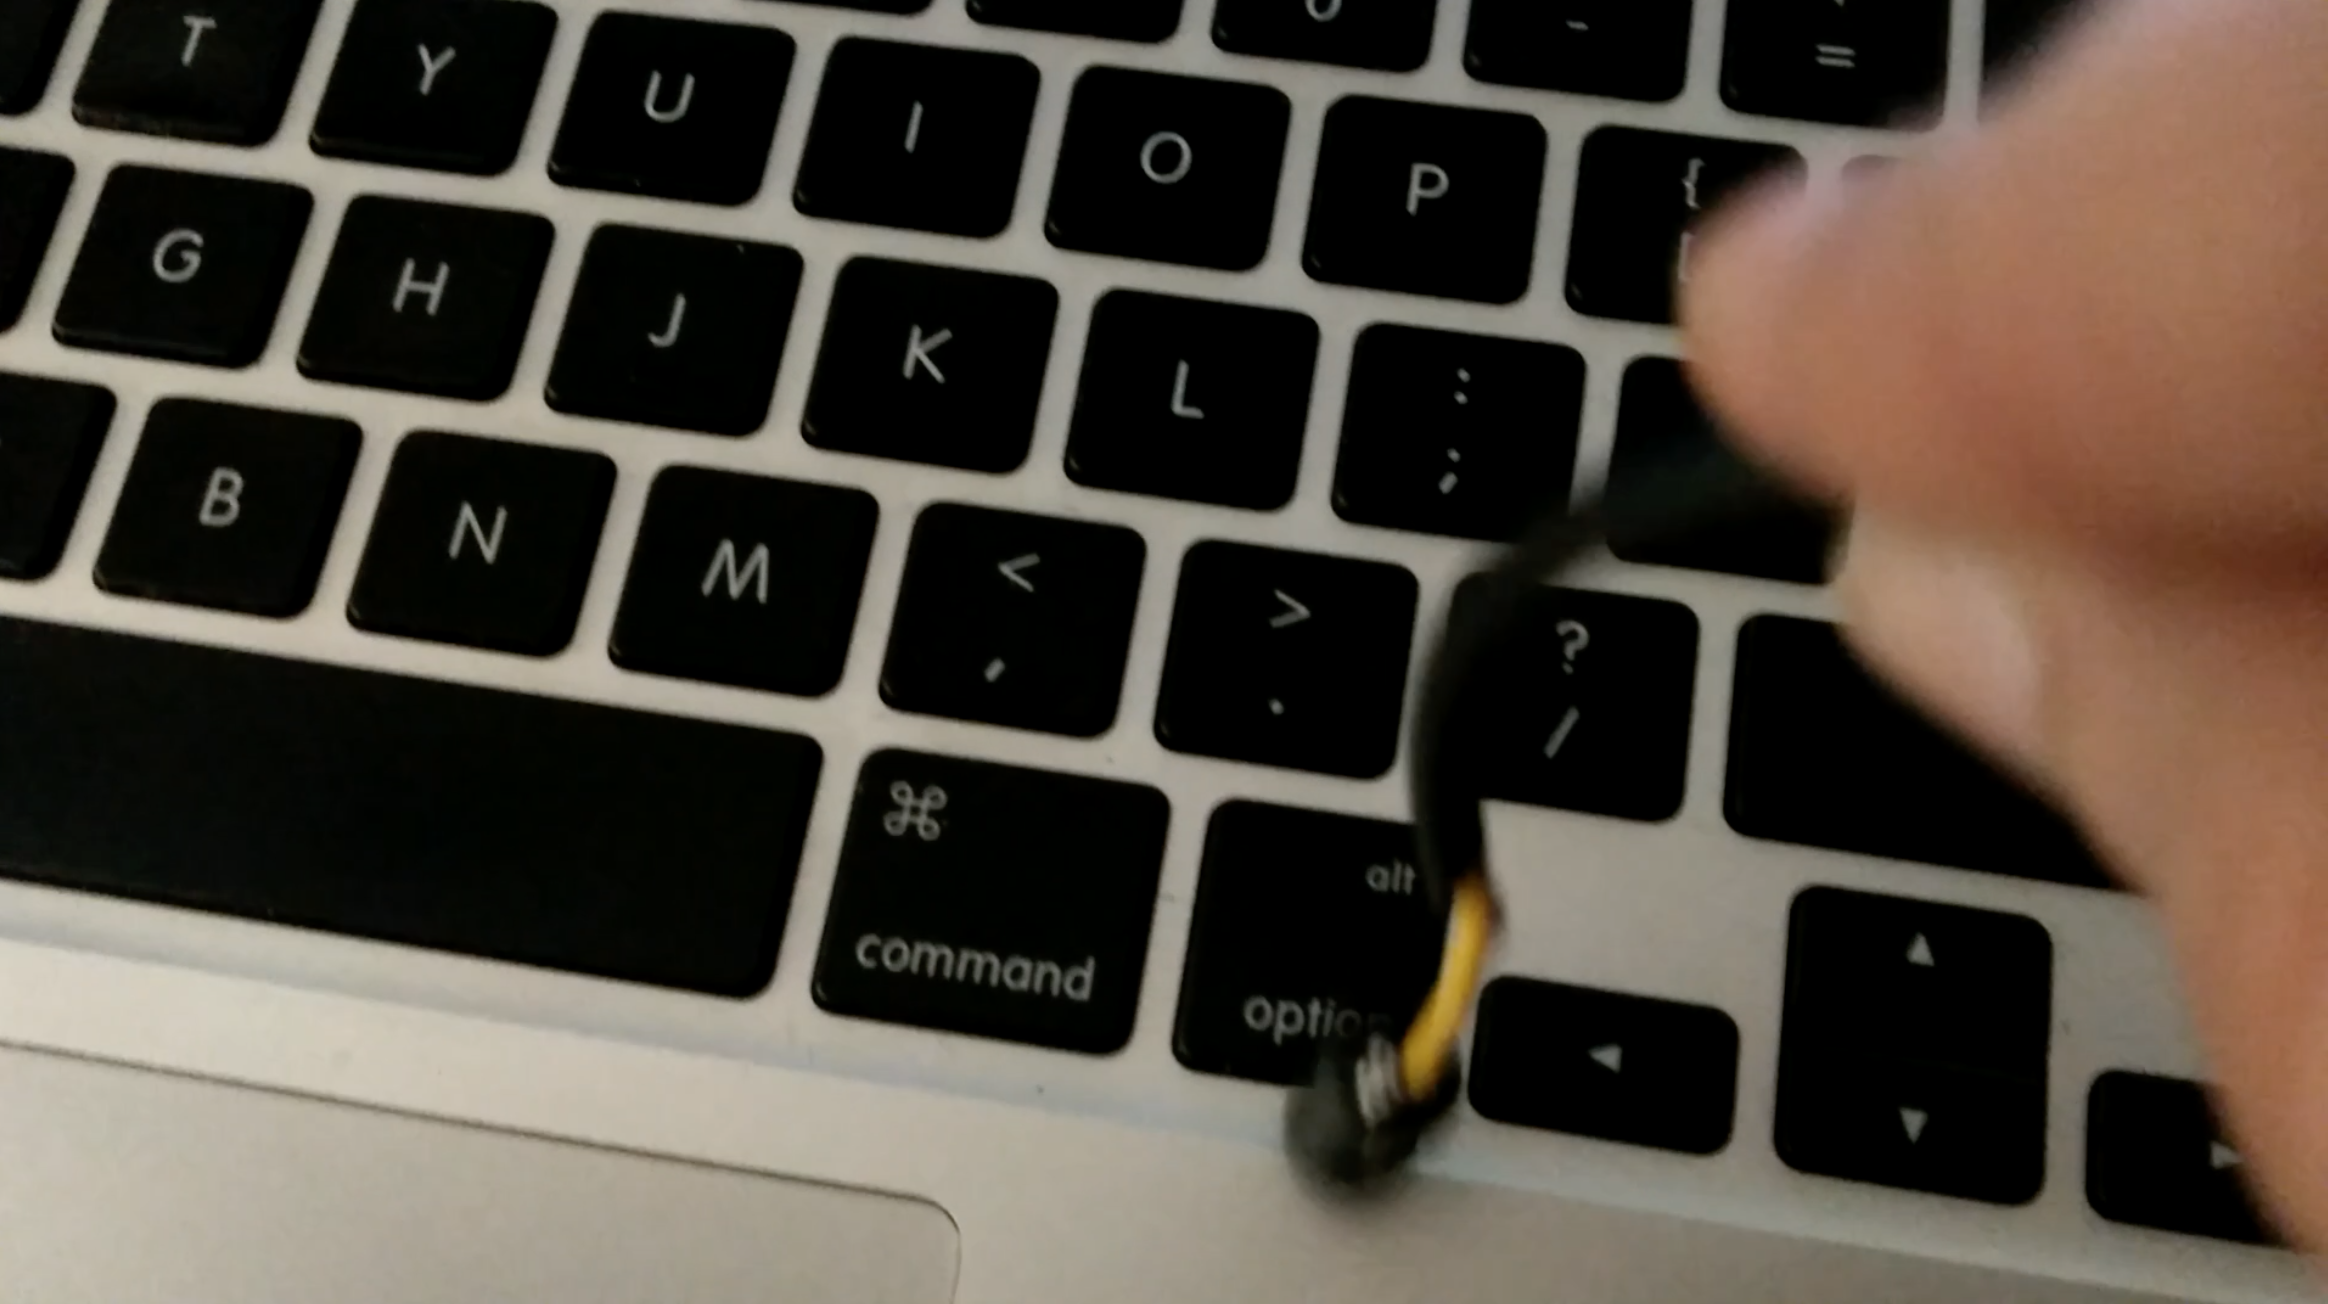
\includegraphics[scale=0.08]{img/pickup.png}
	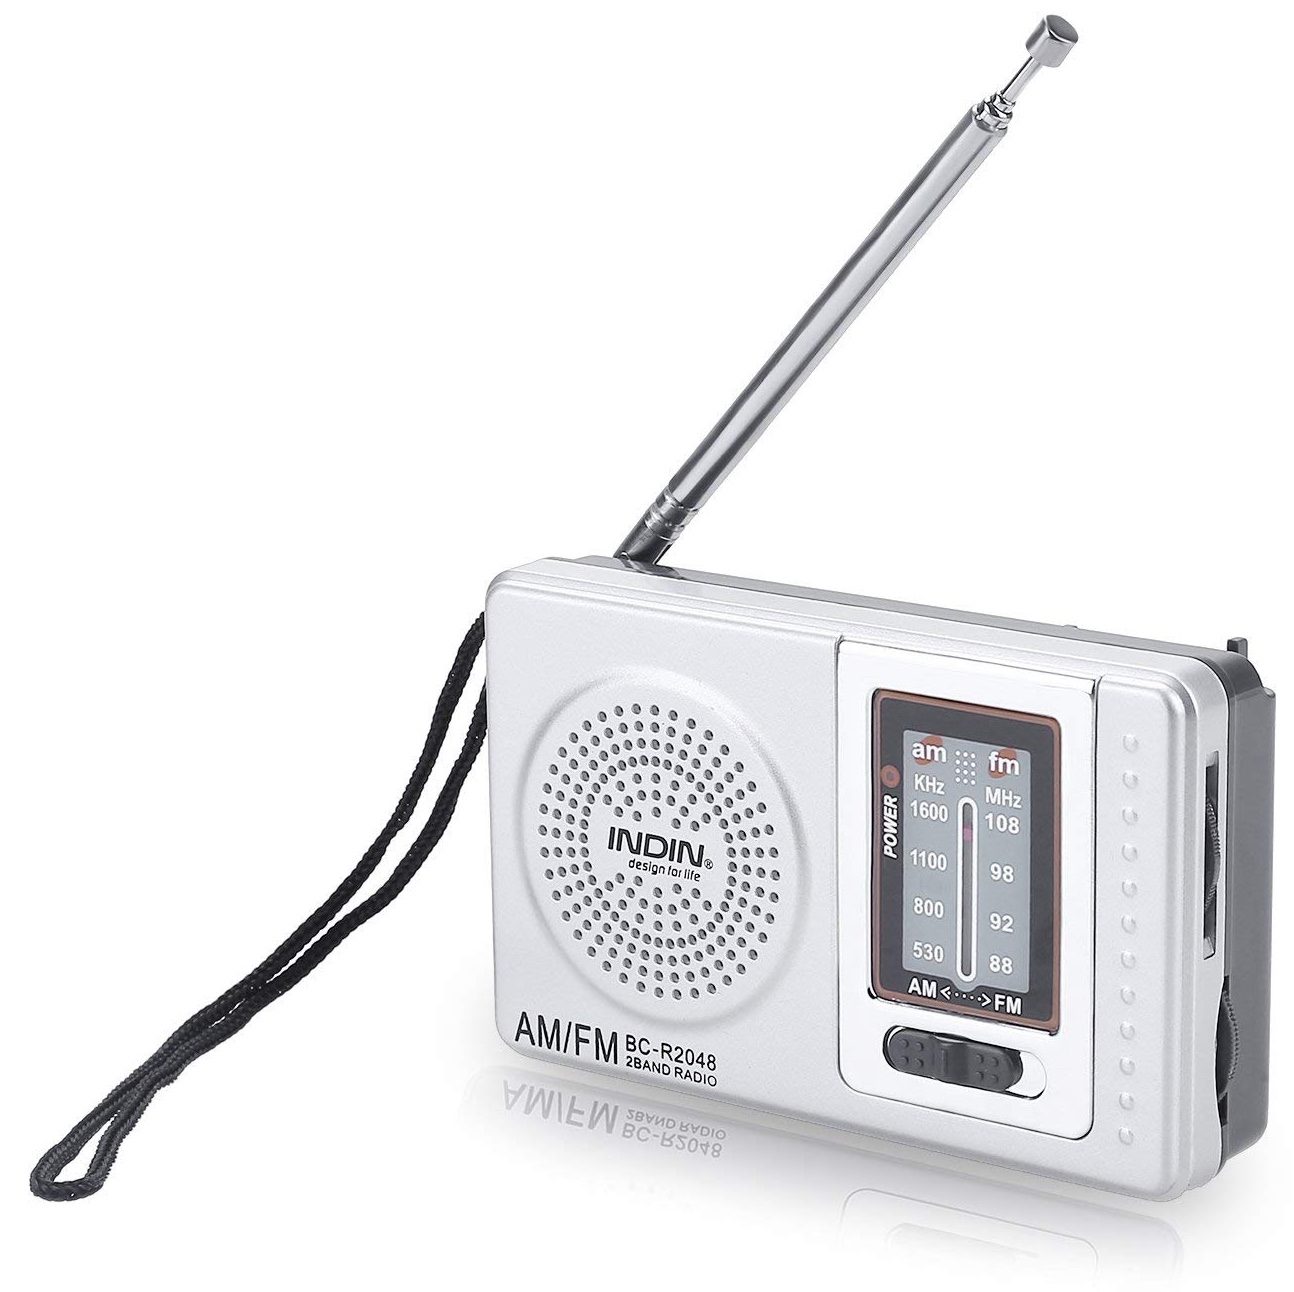
\includegraphics[scale=0.08]{img/battery-powered-radio.jpg}	
\end{figure}
{\scriptsize 
Radios, inductive telephone pickup coils or loose electric guitar pickups capture electromagnetic vibrations and translate them into signals that can be heard through a loudspeaker. We need to find sweet spots of electromagnetic fields.
    \begin{itemize}
	\item If you have an old radio, turn it on. Tune it to a dead spot. Try moving it around various electrical appliances: fluorescent lights, electric motors, computers, cell phones, infrared remote controls. 
	\item Alternatively, a telephone pickup (coil of wire) can act like a radio antenna if plugged into an amp. Use it like a like a stethoscope exploring various electrical appliances: laptops, fans, toys, and so on.
    \end{itemize}   
}    
{\tiny
Exercise based on ``Chapter 3. Circuit sniffing: using radios and coils to eavesdrop on hidden electromagnetic music'' (Collins 2006).
}
\end{frame}
%
\begin{frame}
  \frametitle{Exercise 2: Circuit sniffing}
   \begin{figure}
	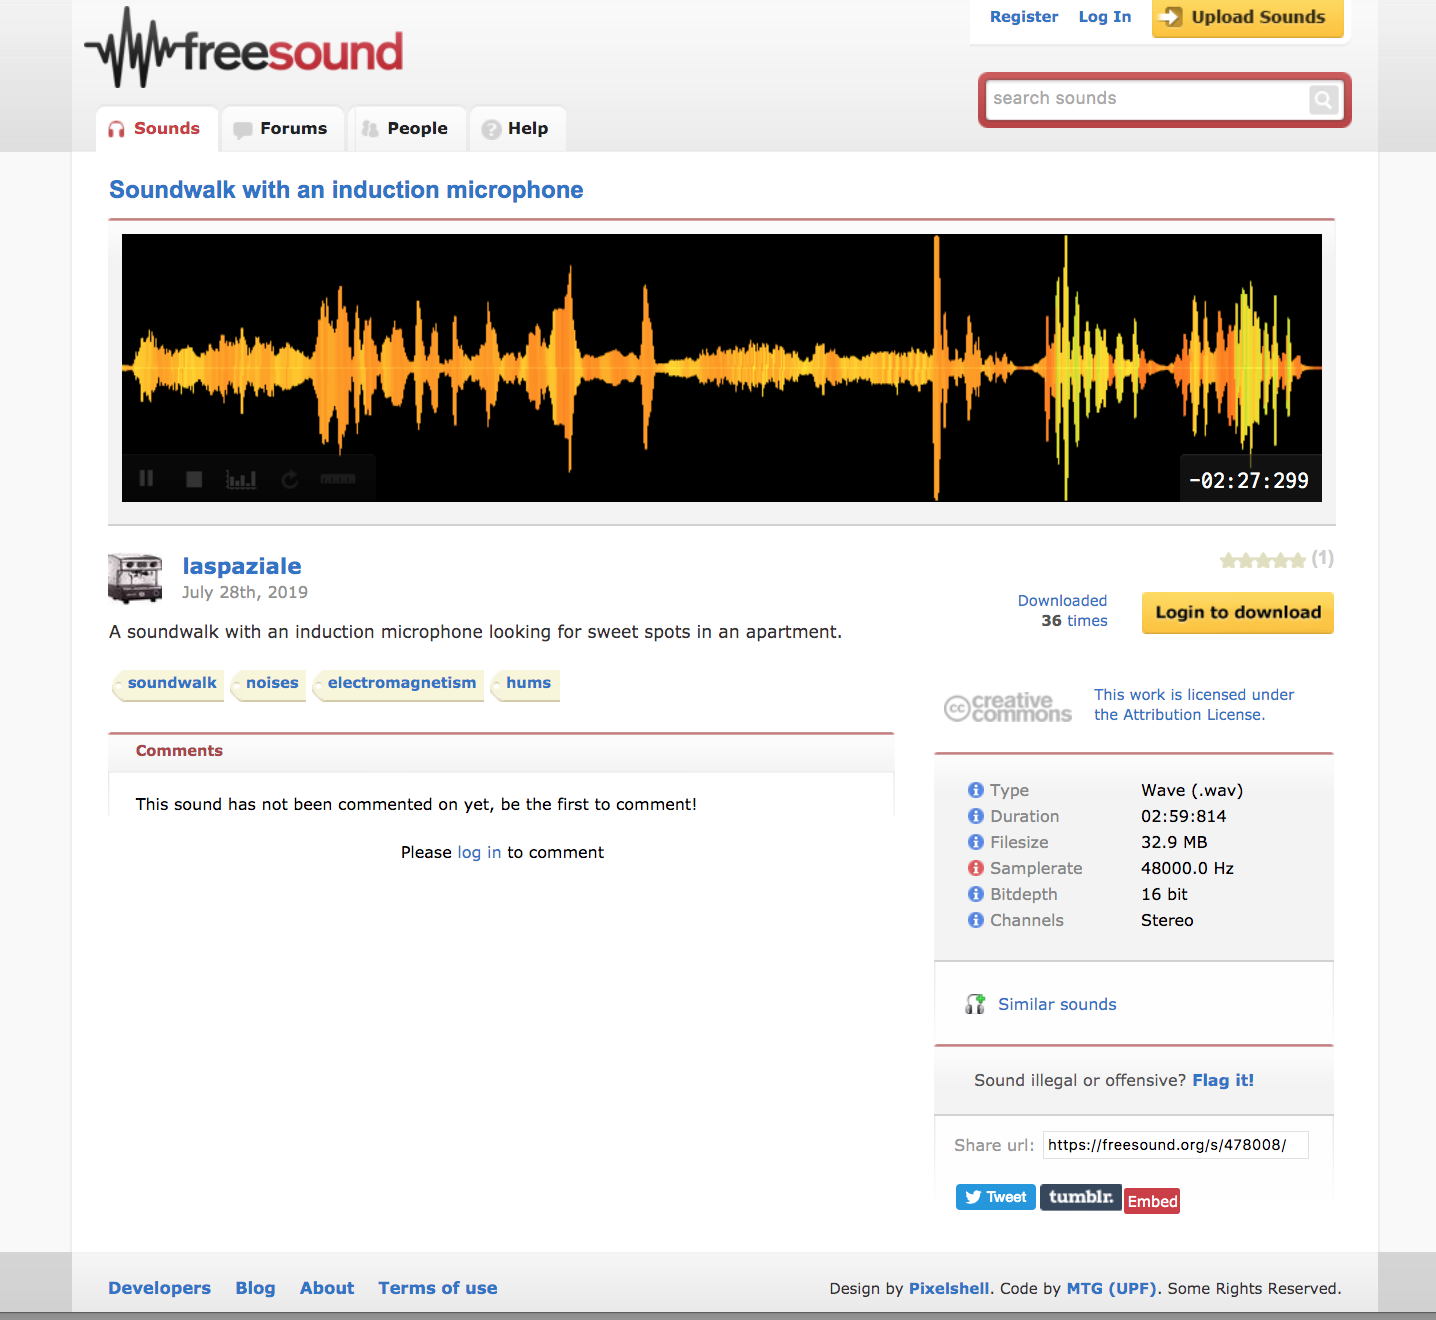
\includegraphics[scale=0.3]{img/Freesound.png}
\end{figure}
{\tiny
\url{https://freesound.org/people/laspaziale/sounds/478008/}
}
\end{frame}
%
\begin{frame}
  \frametitle{Exercise 3: Speaker as a microphone}
 \begin{figure}
	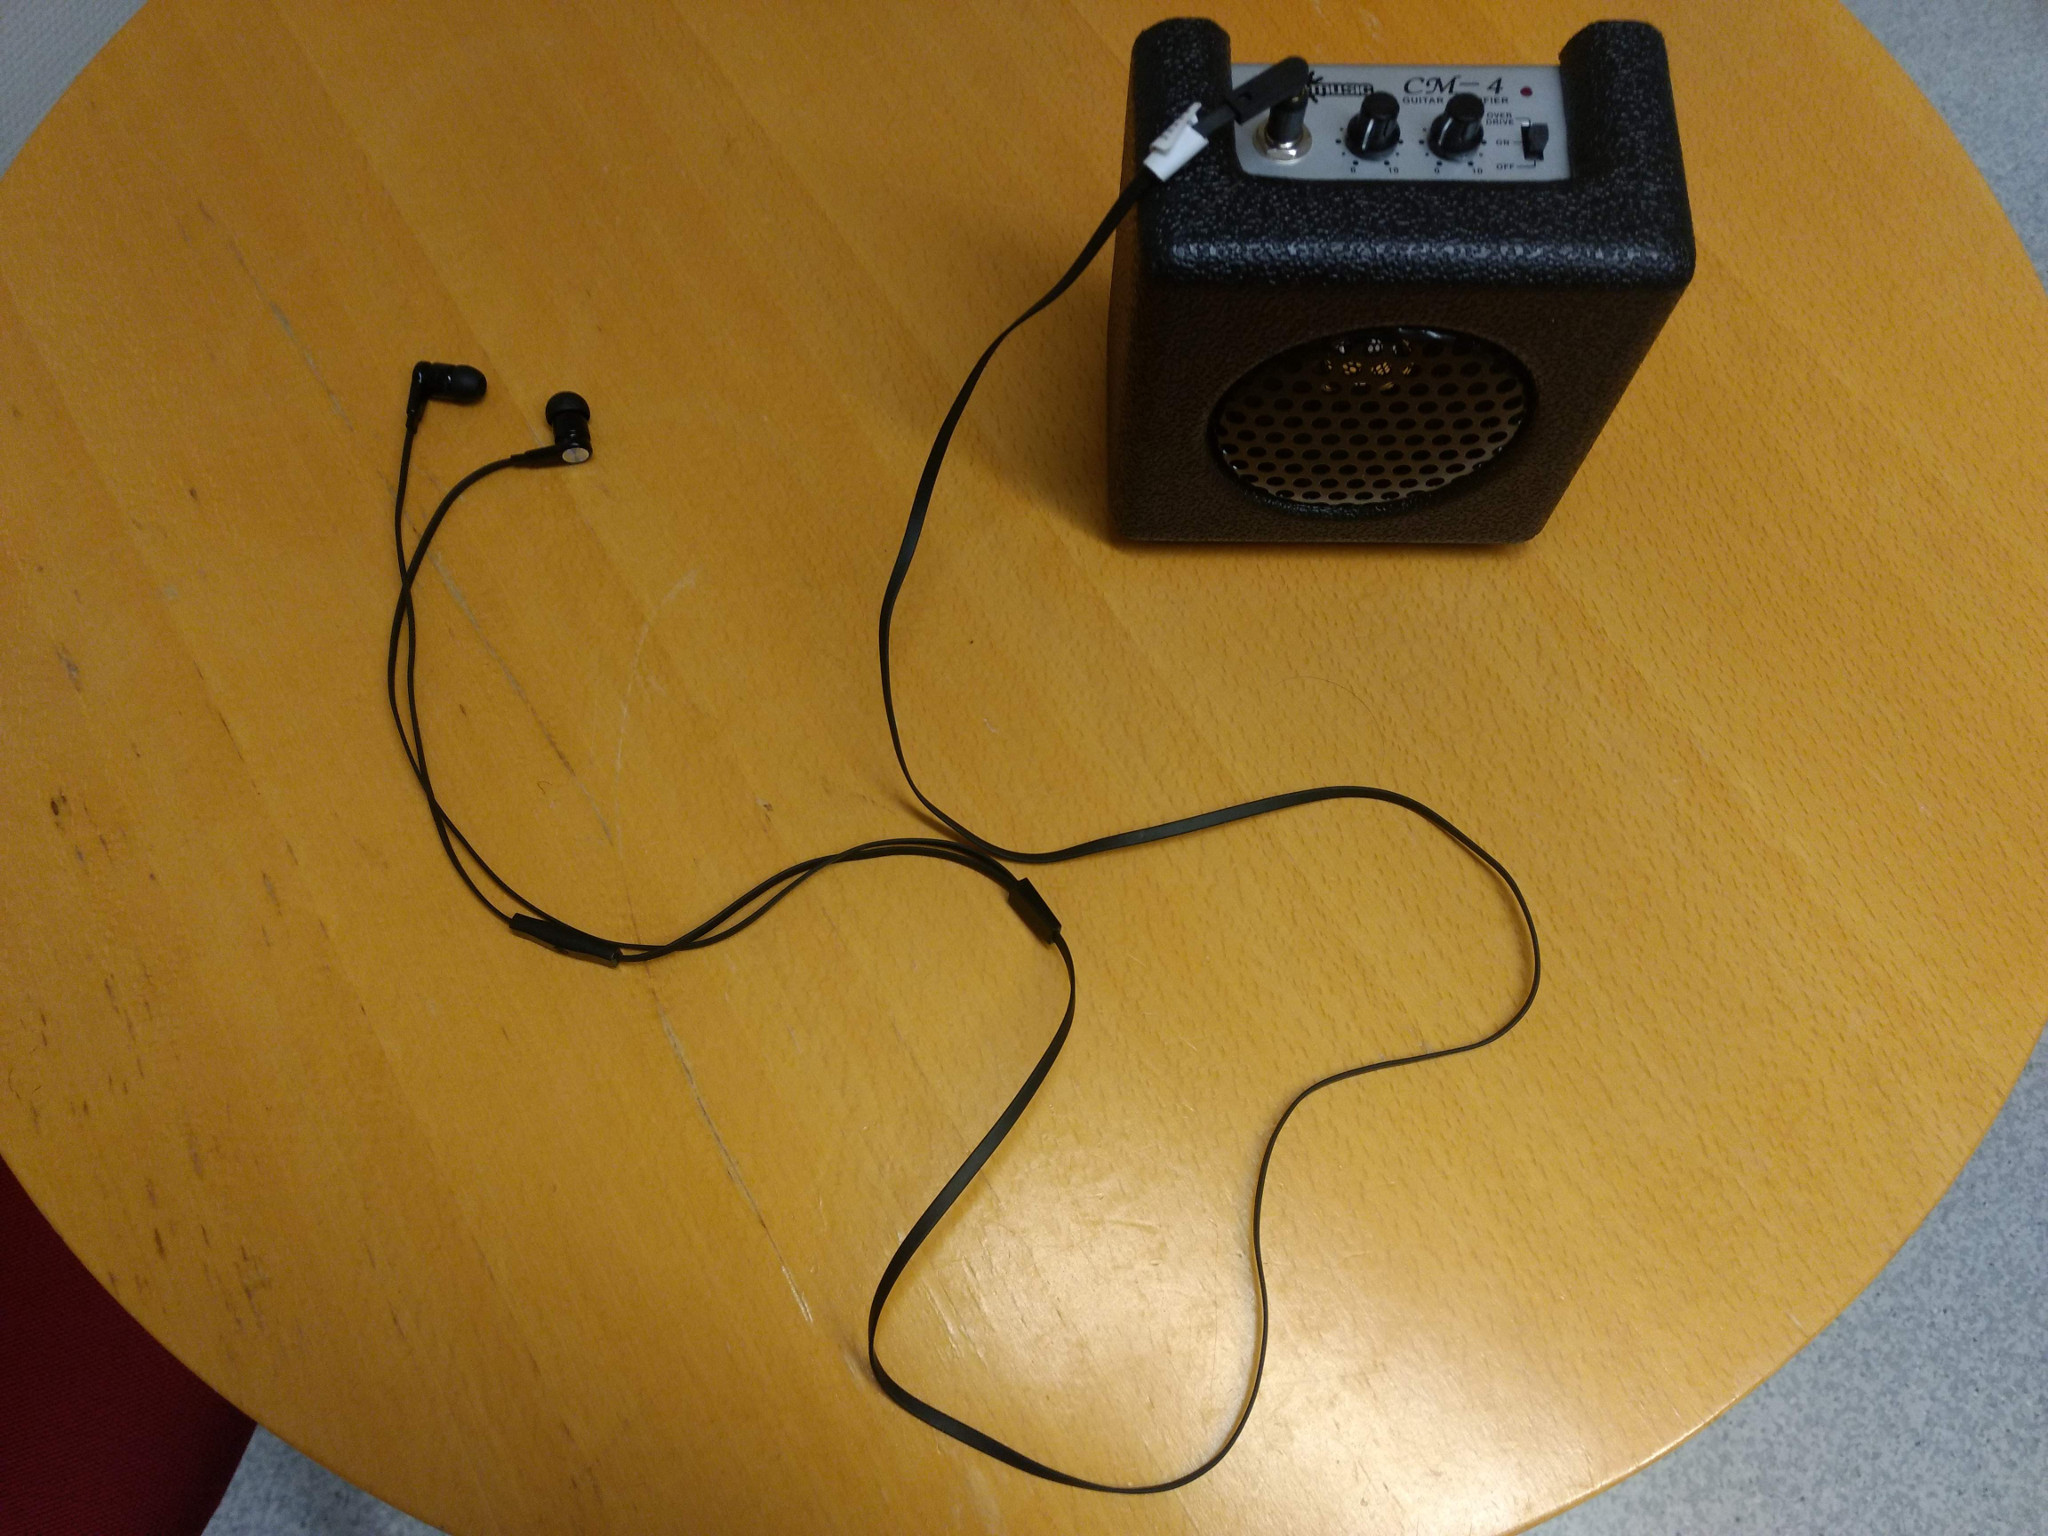
\includegraphics[scale=0.05]{img/coilsamps.jpg}
\end{figure}
{\scriptsize 
Headphones are tiny speakers (both have coils and magnets to transform acoustic sound into an electrical signal or the other way around). The same electromagnetic force is used for both microphones and speakers.
    \begin{itemize}
	\item Try to use headphones as speakers using the circuit sniffing technique.    
    \end{itemize}
 }   
    {\tiny Exercise based on:
     \begin{itemize}
    	\item ``Chapter 4. In/out (the eight rule of hacking): speaker as microphone, microphone as speaker -- the symmetry of it all'' (Collins 2006)
	\item Video ``Tutorial 2: In/Out - Electromagnetism Explained (Chapter 4)'' (source: www.nicolascollins.com)\\ 
	\url{https://www.nicolascollins.com/video/tutorial02/tutorial02-desktop.m4v} 
      \end{itemize}	
    }
       
\end{frame}

%

\begin{frame}
  \frametitle{Exercise 4: Contact mics and amps}
 \begin{figure}
	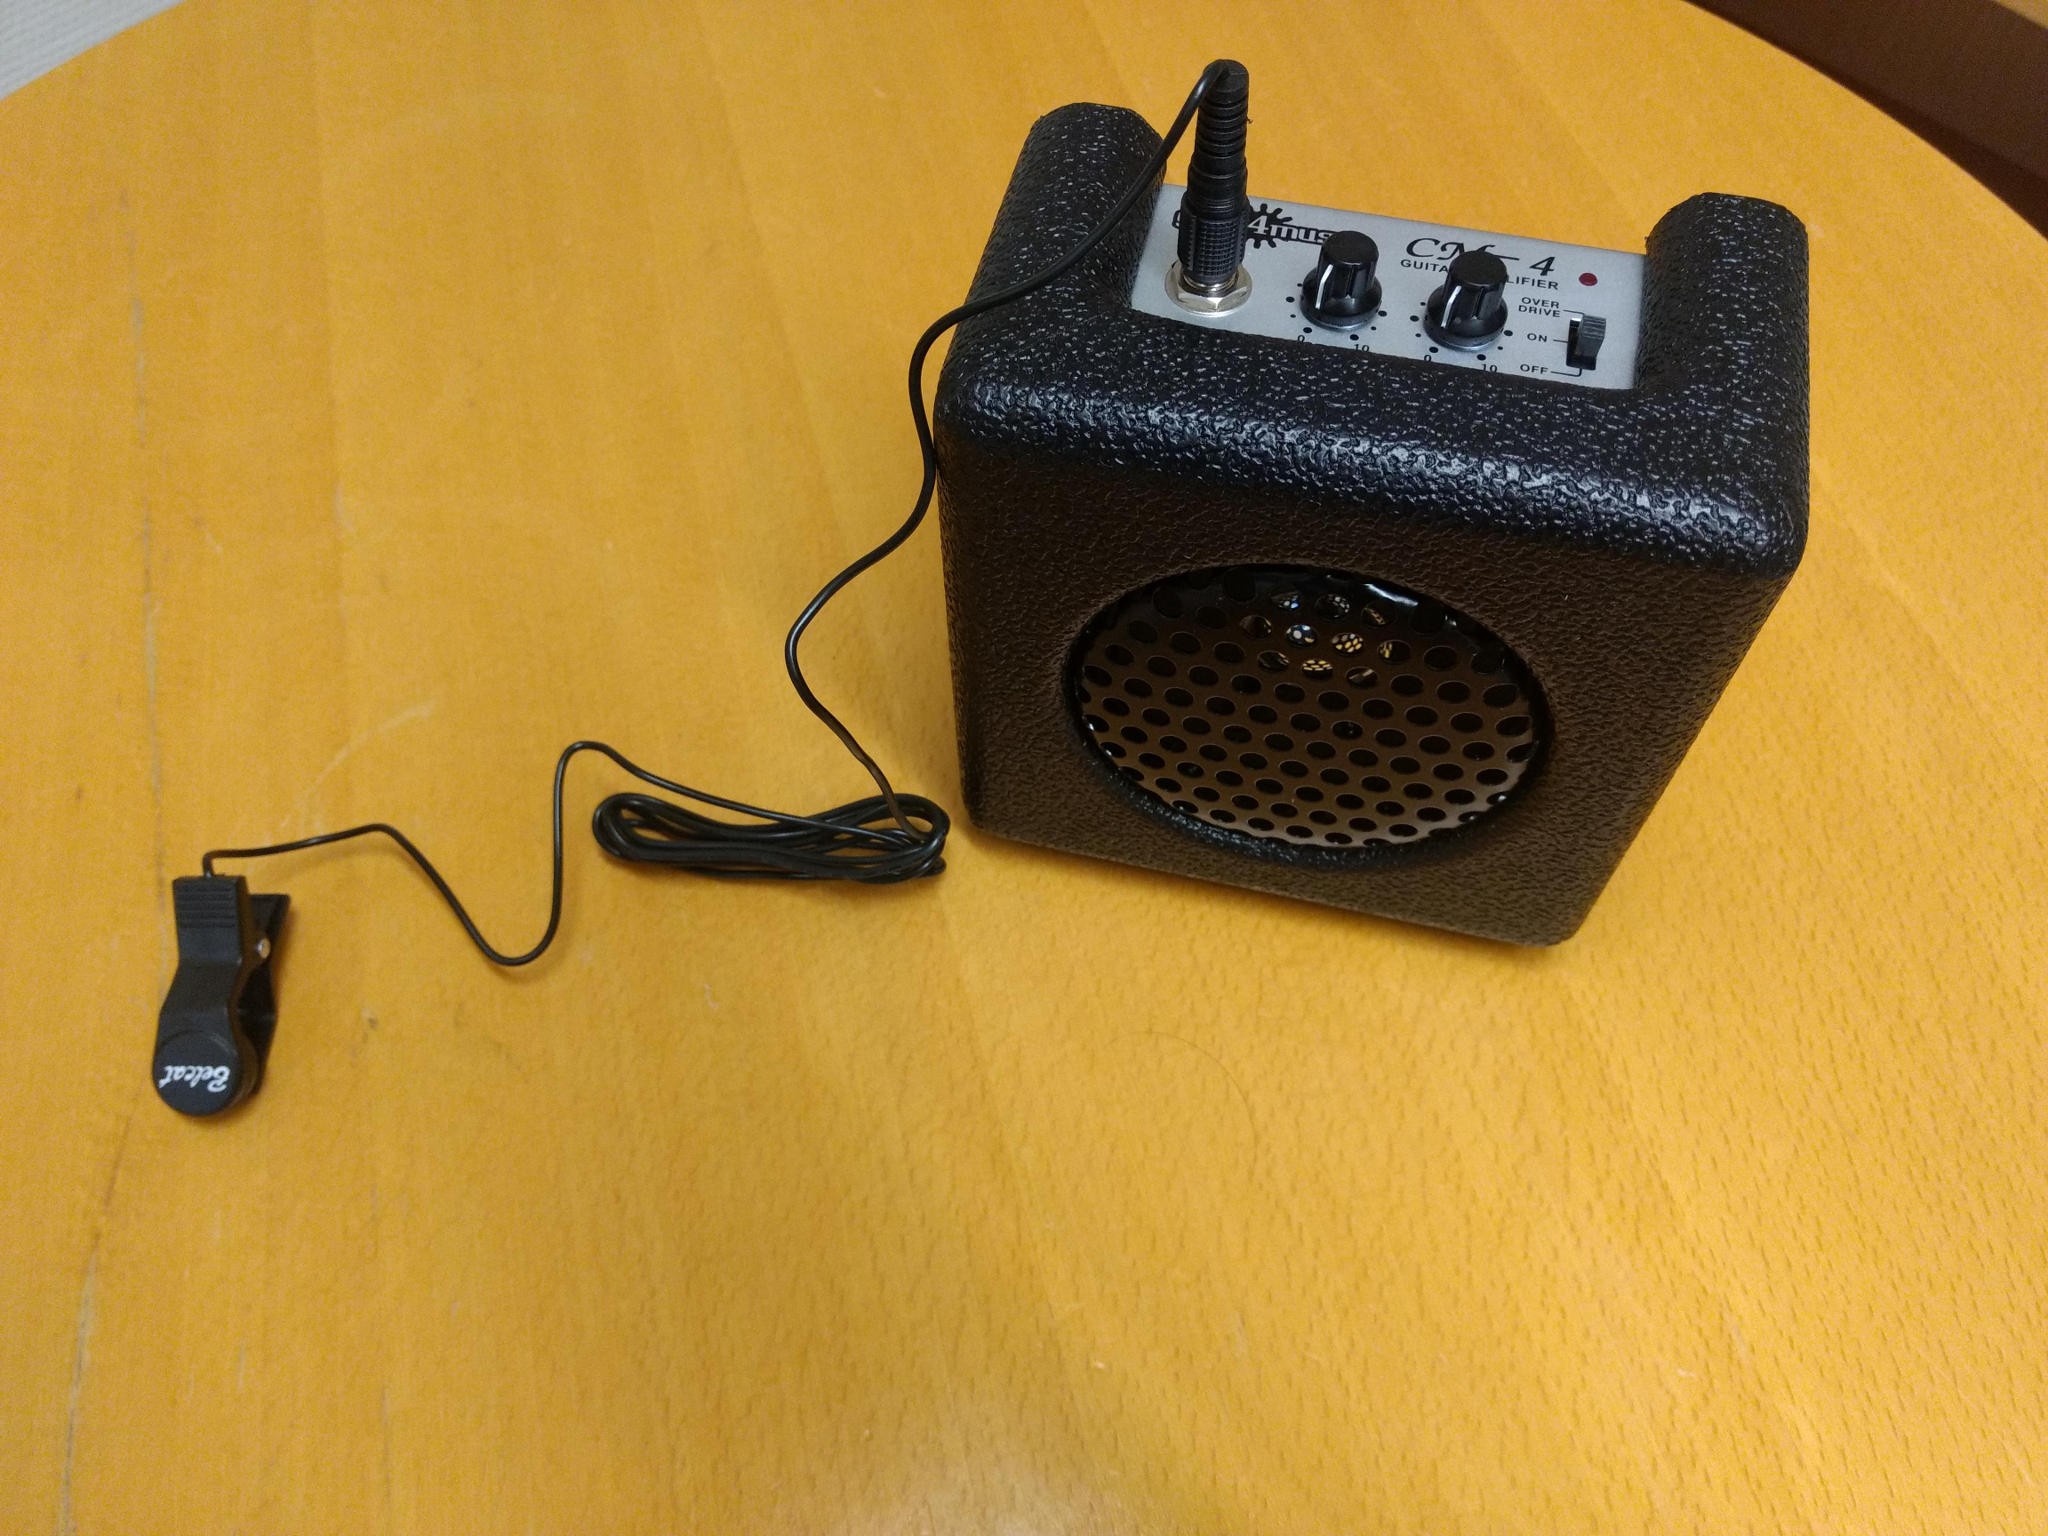
\includegraphics[scale=0.05]{img/contactmics.jpg}
\end{figure}  

  {\scriptsize 
  A contact mic, also known as a pickup or piezo, is a form of microphone that senses audio vibrations through contact with solid objects.
  \begin{itemize}
    \item Go for a soundwalk with contact mics and amps using the circuit sniffing technique. It is recommended to making firm physical contact with the vibrating object. Try: guitars, violins, drums, pots and pans, wrists and knees, foreheads, pinball machines.     
  \end{itemize}
  }
  {\tiny Exercise based on:	  
    \begin{itemize}
	\item ``Chapter 7. How to make a contact mike: Using piezo disks to pick up tiny sounds'' (Collins 2006)
	\item Video ``Tutorial 5: How to Make a Contact Mike (Chapter 7)'' (source: www.nicolascollins.com)\\
	\url{https://www.nicolascollins.com/video/tutorial05/tutorial05-desktop.m4v}
    \end{itemize}
   } 
\end{frame}
%

\usebackgroundtemplate{}
\begin{frame}
\frametitle{}
{\huge Block II\\ Basic Interactive Behavior:\\ Building a Basic Sampler}
\end{frame}

%
\begin{frame}
  \frametitle{A Basic Sampler in Pd Vanilla}
   \begin{figure}
	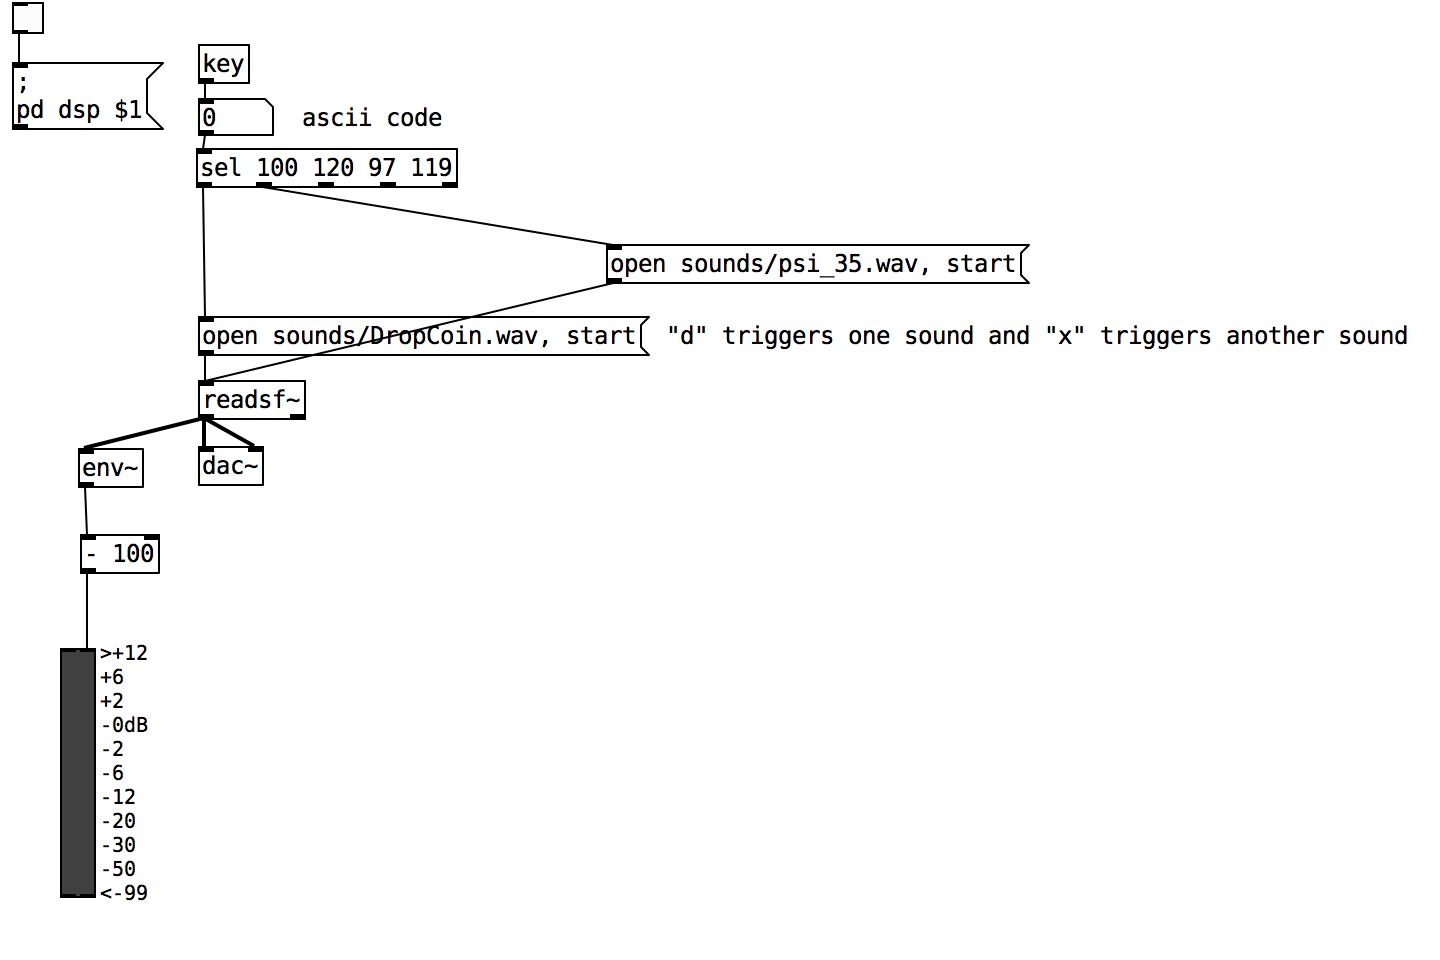
\includegraphics[scale=0.3]{img/Pd-basic-sampler.png}
\end{figure}
{\tiny
\url{https://github.com/axambo/physical-computing-workshop-v2}
}
\end{frame}
%

\usebackgroundtemplate{}
\begin{frame}
\frametitle{}
{\huge Block III\\Fieldwork}
\end{frame}

\begin{frame}
  \frametitle{Fieldwork I: Circuit sniffing + soundwalking activities}
        \begin{itemize}
	\item Generation of audio recordings from soundwalks and circuit sniffing using loudspeakers with batteries, pickup coils, radios, contact mics.
	\item Description of the sounds: action, material, qualities of the sound. 
	\item Selection of the most representative sounds and upload them to Freesound.org.
	\item If suitable, distribution of work between group members ``in the wild'' and group members in the ``station'' e.g. Oslo vs Trondheim or across campuses. 
	\item Writing of a blog post explaining the above process.
    \end{itemize} 
\end{frame}

\usebackgroundtemplate{}
\begin{frame}
\frametitle{}
{\huge Block IV\\Rehearsal and Performance}
\end{frame}



%\begin{frame}
%  \frametitle{Exercise 4: Install P5.js and ``Hello, World''}
% Exercise: Download and familiarize with the code from ``P5\_01\_hello\_world'' project. Print ``Hello, World'' to the javascript console.
% Each student should have a laptop/terminal. In each terminal there should be installed:
%    \begin{itemize}
%	\item A code editor (e.g. Atom, Sublime...).
%	\item A browser.
%	\item Python to run a simple local server (as explained here: \url{https://github.com/processing/p5.js/wiki/Local-server}). 
%	%Mongoose for Windows: https://stackoverflow.com/questions/5050851/best-lightweight-web-server-only-static-content-for-windows
%	\item Internet.
%	\item Optionally: Headphones (if we want to avoid disturbing the other students).
%	\item For each project it will be included P5.js library including p5.sound.js.
%    \end{itemize}
%\end{frame}
%%
%\begin{frame}
%  \frametitle{Exercise 5: A simple sampler in P5.js}
%  Go through the code and exercises from: 
%   \begin{itemize}
%  	\item ``P5\_02\_loadSound''
%	\item ``P5\_03\_loadSound\_playstop\_keyboard'' 
%	\item ``P5\_04\_loadSound\_play\_four\_sounds''
%   \end{itemize}
%  
%  
%\end{frame}
%%
%\begin{frame}
%  \frametitle{Exercise 6: A customized sampler in P5.js}
%  Create your own sampler with today's recordings. Be ready to perform with it!
%\end{frame}
%%
%\begin{frame}
%  \frametitle{Resources: Soundwalks}
%    \begin{itemize}
%	\item Soundwalking as a methodology for understanding soundscapes (paper)\\ 
%	\url{http://usir.salford.ac.uk/2461/1/Adams_etal_2008_Soundwalking_as_Methodology.pdf}
%    \end{itemize}    
%\end{frame}
%%
%\begin{frame}
%  \frametitle{Resources: Circuits}
%    \begin{itemize}
%    \item Basic electricity - What is an ampere / amp? (video): \url{https://www.youtube.com/watch?v=8gvJzrjwjds}
%    \item Circuit fundamentals (video): \url{https://www.youtube.com/watch?v=MusUypbX73Y}
%    %\item How to measure and debug a circuit?
%    %\item Conductive vs non-conductive materials, effects current flow
%    %\item How to draw a circuit? (symbols)
%    %\item Ohm's Law Calculator
%    \end{itemize}    
%\end{frame}
%%
%\begin{frame}
%  \frametitle{Resources: Contact mics}
%    \begin{itemize}
%    	\item Different Types of Transducers in Practical Applications: \url{https://www.efxkits.com/blog/different-types-of-transducers-in-practical-applications/}
%	\item The first rule of CONTACT MIC club: \url{http://www.musicofsound.co.nz/blog/the-first-rule-of-contact-mic-club}
%	\item 9 ways to use piezo mics in your music making: \url{https://www.musicradar.com/tuition/tech/9-ways-to-use-piezo-mics-in-your-music-making-627533}
%	\item Building contact mics: \url{http://maaheli.ee/main/building-contact-microphones/}
%	\item How to use a contact mic for sound design: \url{http://www.synthtopia.com/content/2016/08/15/how-to-use-a-contact-mic-for-sound-design/}
%    \end{itemize}    
%\end{frame}
%%
%\begin{frame}
%  \frametitle{Other Resources: Engineering}
%    \begin{itemize}
%    \item What is Electrical Engineering? \url{https://www.youtube.com/watch?v=QQewdCJTcIU}
%    \item Inspiring the next generation of female engineers \url{https://www.youtube.com/watch?v=FEeTLopLkEo}
%    \end{itemize}
%\end{frame}
%%
%\begin{frame}
%  \frametitle{Other Resources: How to Solder}
%    \begin{itemize}
%    \item ``Chapter 6. How to solder? An essential skill'' (Collins 2006)\\
%    \url{https://www.nicolascollins.com/video/tutorial04/tutorial04-desktop.m4v}     
%    \item How to solder? (video) (source: www.nicolascollins.com)\\
%    \url{https://www.nicolascollins.com/video/tutorial04/tutorial04-desktop.m4v} 
%    \end{itemize}
%\end{frame}
%%
%\begin{frame}
%  \frametitle{Other Resources: Listening}
%    \begin{itemize}
%    \item ``Tutorial 3: Jumping Speakers (Chapter 5)'' (source: www.nicolascollins.com)\\
%    \url{https://www.nicolascollins.com/video/tutorial03/tutorial03-desktop.m4v}
%    \item Alvin Lucier's (USA) ``Sferics'' (1980)\\
%    Audio: \url{https://www.youtube.com/watch?v=rxUvMl_IxoQ}\\
%    About: \url{http://www.alvin-lucier-film.com/sferics.html}
%    \item Karlheinz Stockhausen (Germany), ``Kurzwellen'' (1968) used four receivers in live performance\\
%    Audio: \url{https://www.youtube.com/watch?v=uQ_vGr9U3QY}
%    \item ``Pack: contact microphone recordings'' by klankbeeld\\
%    \url{https://freesound.org/people/klankbeeld/packs/11282/}
%    \end{itemize}
%\end{frame}
%%
%\begin{frame}
%  \frametitle{Other Resources: Listening II}
%    \begin{itemize}
%    \item ``Storytable'' by composer Gyrid Nordal Kaldestad, performed by Architek Percussion (Ben Duinker, Mark Morton, Ben Reimer, Alessandro Valiante):\\
%    \url{https://vimeo.com/184034352}
%    \item Owen Green and his work on cardboard boxes. \\
%    ``Neither the Time Nor the Energy'' (Electric Spring 2018): \url{https://www.youtube.com/watch?v=VExDlHD7o80}
%    \end{itemize}
%\end{frame}
%%
%\begin{frame}
%  \frametitle{References}
%  \printbibliography
%\end{frame}
%
\end{document}
